
%(BEGIN_QUESTION)
% Copyright 2006, Tony R. Kuphaldt, released under the Creative Commons Attribution License (v 1.0)
% This means you may do almost anything with this work of mine, so long as you give me proper credit

Calculate the force generated at the large piston (area = 40 in$^{2}$), given a 25 pound force applied to the small piston (area = 10 in$^{2}$).  Also, calculate the pressures where the two pressure gauges are located, and explain how the hydrostatic pressure of the water column's 20 foot vertical height factors in to this force calculation.

$$\includegraphics[width=15.5cm]{i00159x01.eps}$$

Does the disparity in pressure between the two gauge locations represent a violation of Pascal's Principle?  Why or why not?

\underbar{file i00159}
%(END_QUESTION)





%(BEGIN_ANSWER)

Force at large piston = 100 pounds.

\vskip 10pt

The upper pressure gauge will register 2.5 PSI, and the lower pressure gauge will register 11.17 PSI.

\vskip 10pt

Pascal's Principle may be accurately stated as follows:

\vskip 10pt {\narrower \noindent \baselineskip5pt
``Pressure applied to a confined fluid increases the pressure throughout that fluid volume by the same amount''
\par} \vskip 10pt

Mathematically, we can express Pascal's Principle as follows:

$$\Delta P_1 = \Delta P_2$$

It would be wrong to assume pressure throughout a confined fluid volume is the same (i.e. $\Delta P_1 = \Delta P_2$), because that would preclude hydrostatic pressure which is dependent on height.  It is more accurate to state Pascal's Principle in terms of pressure {\it increase}.

%(END_ANSWER)





%(BEGIN_NOTES)


%INDEX% Physics, fluids: pressure, force, and area
%INDEX% Physics, static fluids: Pascal's Principle

%(END_NOTES)


